% -*- coding: utf-8 -*-
\documentclass[bibieee, standard]{gist} % dense, standard

% Place floats(figures and tables) on a separate page.
\makeatletter % float 전용 페이지의 배치 규칙 설정
\@fpsep\textheight
\makeatother

\makeindex

\input epsf %temporarily inserted for printing figures
\def\putepsf#1{\centering \parbox{12cm}{\epsfxsize = 12cm \epsfbox{#1}}}
%temporarily inserted for printing figures
%-----------------------------------------------------------------------
% ---- Field: Department, Degree ----
\code{{D/}MRE} % {D/}: doctoral, {M/}: master's, {B/}: bachelor's | {DeptCode}: department code
\degreeabbr{PhD} % Printed as <DegreeAbbr>/<DeptCode>, e.g., PhD/MRE
\college{College of Engineering} % YOUR COLLEGE
\kcollege{공과대학} % YOUR COLLEGE NAME
\makeatletter % 학과명 메타데이터 정의, 그래서 표지/제출서/초록 앞부분 페이지에 직접 반영
\def\@edept{Department of Mechanical and Robotics Engineering} % Department full name (EN)
\def\@kdept{기계로봇공학과} % Department full name (KR)
\def\@kdeptn{기 계 로 봇 공 학 과} % Department full name with space (KR)
\makeatother

%-----------------------------------------------------------------------
% ---- Field: Thesis title (EN, KR) ----
% Insert \titlebreak where lines are to be separated.  Do not use the LaTeX command '\\'.
\etitle{ENGLISH THESIS TITLE HERE}
\ktitle{한 글 논 문 제 목 입 력}


%-----------------------------------------------------------------------
% ---- Field: Advisor, Co-advisor ----
\advisor{John Smith} % Advisor's name in English without a position such as 'Prof.'.
\kadvisor{홍길동} % Advisor's name in Korean without a position such as 'Prof.'.
%\coadvisor{} % Co-advisor's name in English without a position such as 'Prof.'.
% ---- Field: Author, Referees ----
\ename{Richard Roe} % Name of the author in English
\kname{{김}{철}{수}} % Name of the author in Korean separated with '{}'.
% ---- Field: Referees ----
\studentid{000000} % 6-digit Student ID of the author
\coveryear{2026}  % The year of graduation, YYYY
\advisorsigndate{June}{1}{2026}% The date signed by the advisor, MM/DD/YYYY
\refereesigndate{June}{1}{2026} % The date signed by the referees, MM/DD/YYYY
%-----------------------------------------------------------------------

%-----------------------------------------------------------------------
% Names of the referees in English
\refereeA{Prof. John Smith} % Advisor
\refereeB{Prof. John Doe}   % Committee member
\refereeC{Prof. Jane Doe}   % Committee member
% \refereeD{Prof. }  % Committee member
% \refereeE{Prof. } % Committee member

%-----------------------------------------------------------------------
\dedication{Dedicated to my family.} % beginning of thesis.
\hypersetup{pageanchor=false} % avoid duplicate PDF page destinations across frontmatter/mainmatter resets
\begin{document}

%-----------------------------------------------------------------------
% Abstract
\begin{eabstract} This dissertation template provides a minimal starting point for writing a thesis with the GIST class. The placeholder text in this repository is intentionally generic so that authors can replace each section with their own research content without first reorganizing the document structure.

This sample abstract demonstrates the expected tone and composition of an English abstract. A typical abstract briefly states the research background, defines the problem, summarizes the proposed approach, and closes with the main findings and contributions. The exact content should be concise, self-contained, and understandable without requiring the reader to consult the main chapters.

Keywords: thesis template, dissertation, LaTeX, placeholder, academic writing
 \end{eabstract} % in english
\begin{kabstract} 이 논문 템플릿은 GIST 학위논문 양식을 기준으로 작성되었으며, 사용자가 전체 문서 구조를 다시 설계하지 않고도 바로 원고를 작성할 수 있도록 예시용 내용을 포함한다. 배포용 저장소의 목적상 각 장과 절의 문장은 특정 연구 주제에 종속되지 않도록 중립적으로 구성하였다.

이 초록 예시는 국문 초록에 포함될 수 있는 기본 요소를 보여준다. 일반적으로 초록에는 연구 배경, 문제 정의, 접근 방법, 핵심 결과, 그리고 학술적 기여가 간결하게 정리된다. 실제 제출본에서는 연구 분야에 맞는 용어와 정량적 결과를 반영하여 내용을 수정하면 된다.

 \end{kabstract} % in korean
% \begin{acknowledgements} I would like to thank my advisor, committee members, colleagues, friends, and family for their support throughout this work. This file is optional and may be removed or replaced depending on the submission requirements of the department.
 \end{acknowledgements} % Acknowledgements

%-----------------------------------------------------------------------
\makecontents % Table of contents
\listtables % List of tables (comment out if there is no table)
\listfigures % List of figures (comment out if there is no figure)

%-----------------------------------------------------------------------
% Main body of the thesis.  Insert \chapter{Chapter Title} to start a new chapter.
\hypersetup{pageanchor=true}
\pagenumbering{arabic} % generate page number in arabic numerals (1, 2, 3, ...)
\setcounter{page}{1} % start page number from 1

% ---- Thesis Body ---- %
\chapter{Introduction}

This repository is distributed as a thesis-formatting starter project. The introduction chapter can be used to present the research background, define the problem scope, summarize the motivation, and explain the overall organization of the dissertation.

\section{Background}

Most dissertations begin by situating the topic within a broader academic or engineering context. This section is a suitable place to describe prior developments, explain why the problem matters, and identify the limitations of existing approaches. When adapting this placeholder, the author can replace the generic discussion with literature-grounded statements and appropriate citations.

\section{Research Objective}

The objective of this sample chapter is not to communicate a real research claim, but to show a clean structure that can be edited with minimal effort. A practical objective statement usually answers three questions: what problem is being solved, what method is being proposed, and what outcome is expected from that method~\cite{abbott2015}.

\section{Document Organization}

The remainder of this template is organized as follows. Chapter~I illustrates basic figure placement and a preferred subfigure macro. Chapter~II provides an additional chapter placeholder that may be used for methods, experiments, or discussion. The summary section then demonstrates a concise concluding structure.

\chapter{Chapter I}

This chapter demonstrates placeholder body text, figure insertion, subfigure usage, and cross-referencing. In an actual dissertation, this chapter could correspond to a methodology chapter, a theoretical framework, or the first major technical contribution.

\section{Example Figure Layout}

The first example below shows a standard two-image layout using plain \verb|\includegraphics| commands. This is useful when subcaptions are unnecessary and only a single caption is needed for the combined visual result.


\begin{figure}[t]
    \centering
    
\includegraphics[width=0.45\textwidth]{figs/cat1}\hfill
    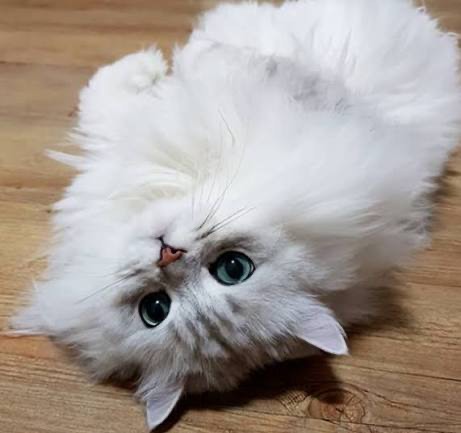
\includegraphics[width=0.45\textwidth]{figs/cat2}
    \caption{Cats}
    \label{fig:cats}
\end{figure}

Figure~\ref{fig:cats} is intentionally simple and serves as a quick reference for authors who only need a single caption for multiple images.

\section{Example Subfigure Macro}

% Subfigure macro
% \subfig[Caption]{Size}{Fig_Path}{Label}
\begin{figure}[t]
    \centering
    \subfig[Cat1.]{0.45\textwidth}{figs/cat1}{fig:cat2_1}
    \hfill
    \subfig[Cat2.]{0.45\textwidth}{figs/cat1}{fig:cat2_2}
    \caption{Cats! with subfig macro}
    \label{fig:cats2}
\end{figure}

The preferred macro example is shown in Figure~\ref{fig:cats2}. Subfigure references can be written directly in the text, for example as Cat1~\ref{fig:cat2_1} and Cat2~\ref{fig:cat2_2}. This pattern is useful when separate discussion is needed for each panel while preserving one shared figure environment.

\section{How To Reuse This Chapter}

For distribution purposes, this chapter is intentionally generic. Authors may replace the section titles, captions, labels, and body text while retaining the overall formatting pattern. If the project is shared with new users, keeping at least one working figure example in the template tends to reduce setup friction.

\chapter{Chapter II}

This chapter provides a second content placeholder for users who want to verify the multi-chapter flow of the template. In a real manuscript, this location could be used for experimental setup, results, discussion, or a case study.

\section{Example Section}

Long-form technical writing usually benefits from a chapter structure that separates assumptions, methods, and evaluation. Even when the final chapter titles differ, starting from a stable outline makes it easier to maintain page numbering, figure numbering, and table references across the full document.

\section{Example Table}

Table~\ref{tab:placeholder} shows a minimal table environment that can be copied and extended.

\begin{table}[t]
    \centering
    \caption{Placeholder comparison table}
    \label{tab:placeholder}
    \begin{tabular}{lcc}
        \hline
        Item & Value A & Value B \\
        \hline
        Example 1 & 10 & 12 \\
        Example 2 & 15 & 18 \\
        Example 3 & 21 & 20 \\
        \hline
    \end{tabular}
\end{table}

\section{Discussion Placeholder}

This section may be replaced with interpretation of results, error analysis, limitations, or comparison with prior work. The main purpose of the current text is to show that chapter-level prose, figures, tables, and references can coexist cleanly in the distributed template.

% ---- Thesis Body ---- %


\summary{tex/5_summary.tex} % dissertation summarization, conclusion.

% \chapter{PLRC and ADE implementations of Drude-critical point model for the FDTD method}
% \label{ch:dcp}
% \input tex/content/dcp.tex

% \chapter{Examples of GMES}
% \label{ch:example}
% \input tex/content/example.tex

% \chapter{Summary}
% \label{ch:summary}
% \input tex/5_summary.tex

% \appendix
% \chapter{How to get GMES}
% \label{ch:get_gmes}
% \input tex/content/get_gmes.tex

%-----------------------------------------------------------------------
% This is the end of the main thesis body.

%-----------------------------------------------------------------------
% bibliography file here.
\gistbibliography{thesis}

\printindex

%-----------------------------------------------------------------------
\birthday{January}{1}{2000}
\birthplace{Sample City, Country}
\addr{123 Example Street, Sample District, Sample City, Country}

\vitae
\begin{education}{20XX.03--20XX.08}
    \item[20XX.03--20XX.08] Department Name, \\University Name (Ph.D.)
    \item[20XX.03--20XX.02] Department Name, \\University Name (M.Sc.)
    \item[20XX.03--20XX.02] Department Name, \\University Name (B.S.)
\end{education}

% \begin{experience}{1cm}
%     \item[20XX.08--20XX.12] Example research and development role, Example Research Center
%     \item[20XX.07--20XX.12] Example engineering project, Example Laboratory
% \end{experience}

\begin{award}
    \item Example scholarship or academic award
\end{award}

\begin{publication}{1cm}
    % \item[]\hspace{-\labelwidth}\hspace{-\labelsep}\textbf{Computer software}:
    % \item[1.] \textbf{Author}, Example Software (Institution Name, 20XX).

    % \item[]\hspace{-\labelwidth}\hspace{-\labelsep}\textbf{Translations}:
    % \item[1.] Author A, Author B, and Author C, \textit{``Title of the translated work,''} (Publisher Name, 20XX).

    % \item[]\hspace{-\labelwidth}\hspace{-\labelsep}\textbf{Book chapters}:
    % \item[1.] \textbf{A. Author}, B. Author, and C. Author, ``Title of the book chapter,'' in \textit{Book Title}, E. Editor and F. Editor, Eds. (Publisher Name, 20XX), pp.~xx--xx.

    \item[]\hspace{-\labelwidth}\hspace{-\labelsep}\textbf{Journals}:
    \item[1.] Author, ``Title of the journal article,'' \textit{Journal Name}, vol.~x, no.~x, pp.~xx--xx, year.

    % \item[]\hspace{-\labelwidth}\hspace{-\labelsep}\textbf{International conferences}:
    % \item[1.] A. Author, \textbf{B. Author}, and C. Author, ``Title of the international conference paper,'' in \textit{International Conference Name} (20XX), pp. xx--xx.

    % \item[]\hspace{-\labelwidth}\hspace{-\labelsep}\textbf{Domestic conferences}:
    % \item[1.] \textbf{A. Author}, B. Author, and C. Author, ``Title of the domestic conference paper,'' in \textit{Domestic Conference Name} (20XX), pp. xx--xx.

    % \item[]\hspace{-\labelwidth}\hspace{-\labelsep}\textbf{Magazines}:
    % \item[1.] \textbf{Author}, ``Title of the magazine article,'' \textit{Magazine Name} pp.~xx--xx (20XX).

\end{publication}

\begin{cvpatents}
    \item \textbf{Example Patent Title}, Country or Office, status or number.
\end{cvpatents}


%-----------------------------------------------------------------------
% This is the end of the thesis.
%
\end{document}
